\documentclass[11pt]{book}
\usepackage[subpreambles=true]{standalone}
\usepackage[spanish]{babel}
\usepackage{comfortaa}
\usepackage[T1]{fontenc}
\usepackage[utf8]{inputenc}
\usepackage[
letterpaper,
left=1in, 
right=1in, 
top=1in,
bottom=1in,
headheight=10mm,% Set \headheight to 10mm
]{geometry} % Custom margins
\usepackage{float}
\usepackage{fancyhdr}
\usepackage{color, colortbl}
\usepackage[dvipsnames,table]{xcolor} % Required for custom color
\usepackage[colorlinks = true, linkcolor = colorrds]{hyperref}
\usepackage{bookmark}
\usepackage{graphicx}
\usepackage{tabularx}
\usepackage{multicol,multirow}
\usepackage{newclude}
%\usepackage{tabto}
\usepackage{remreset}
\usepackage[inline]{enumitem}
\usepackage{xparse}
\usepackage{wrapfig}
\usepackage{caption}
\usepackage{amssymb,amsmath}
\usepackage{tikz}
\usepackage{etoolbox}
\usepackage{ragged2e}
\usepackage{pdflscape}
\usepackage{subfiles} % Best loaded last in the preamble
\input{insbox}
\usepackage[many]{tcolorbox}
% \usepackage{mathspec} 			    % for FONTS
% \usepackage{setspace}               % for LINE SPACING
% \setmainfont{Noto Sans}[
%     Kerning = On,
%     Mapping = tex-text,
%     Numbers = Uppercase,
%     BoldFont = Noto Sans SemiBold
% ]                           % setting the font as Noto Sans
% \setlength\parindent{0pt}   % killing indentation for all the text
% \setstretch{1.3}            % setting line spacing to 1.3
% \setlength\columnsep{0.25in} % setting length of column separator
% \pagestyle{empty}           % setting pagestyle to be empty


\definecolor{main}{HTML}{5989cf}    % setting main color to be used
\definecolor{sub}{HTML}{cde4ff}     % setting sub color to be used

\tcbset{
    sharp corners,
    colback = white,
    before skip = 0.2cm,    % add extra space before the box
    after skip = 0.5cm      % add extra space after the box
}                           % setting global options for tcolorbox


\newtcolorbox{bA}{
    %sharpish corners, % b
    enhanced,
    %colback = sub, % background color
    boxrule = 0.2pt,  % no borders
    %borderline = {1pt}{1pt}{black!35}, % add "dashed" for dashed line
    %fontupper = \bf\color{black}, % font color
    %colframe = main % frame color
    rounded corners,
    %arc = 5pt,   % corners roundness
    fuzzy shadow = {2pt}{-4pt}{-1pt}{1pt}{black!35}, % {xshift}{yshift}{offset}{step}{options} 
    %toprule = 3pt, % top rule weight
    %bottomrule = 3pt % bottom rule weight
}
% You can copy any following box you like to your code.
\newtcolorbox{boxA}{
    fontupper = \bf,
    boxrule = 1.5pt,
    colframe = black % frame color
}

\newtcolorbox{boxB}{
    fontupper = \bf\color{main}, % font color
    boxrule = 1.5pt,
    colframe = main,
    rounded corners,
    arc = 5pt   % corners roundness
}

\newtcolorbox{boxC}{
    colback = sub, % background color
    boxrule = 0pt  % no borders
}

\newtcolorbox{boxD}{
    colback = sub,
    colframe = main,
    boxrule = 0pt,
    toprule = 3pt, % top rule weight
    bottomrule = 3pt % bottom rule weight
}

\newtcolorbox{boxE}{
    enhanced, % for a fancier setting,
    boxrule = 0pt, % clearing the default rule
    borderline = {0.75pt}{0pt}{main}, % outer line
    borderline = {0.75pt}{2pt}{sub} % inner line
}

\newtcolorbox{boxF}{
    colback = sub,
    enhanced,
    boxrule = 1.5pt,
    colframe = white, % making the base for dash line
    borderline = {1.5pt}{0pt}{main, dashed} % add "dashed" for dashed line
}

\newtcolorbox{boxG}{
    enhanced,
    boxrule = 0pt,
    colback = sub,
    borderline west = {1pt}{0pt}{main},
    borderline west = {0.75pt}{2pt}{main},
    borderline east = {1pt}{0pt}{main},
    borderline east = {0.75pt}{2pt}{main}
}

\newtcolorbox{boxH}{
    colback = colorrds!10,
    colframe = colorrds,
    boxrule = 0pt,
    leftrule = 6pt % left rule weight
}

\newtcolorbox{boxI}{
    colback = sub,
    colframe = main,
    boxrule = 0pt,
    toprule = 6pt % top rule weight
}

\newtcolorbox{boxJ}{
    sharpish corners, % better drop shadow
    colback = sub,
    colframe = main,
    boxrule = 0pt,
    toprule = 4.5pt, % top rule weight
    enhanced,
    fuzzy shadow = {0pt}{-2pt}{-0.5pt}{0.5pt}{black!35} % {xshift}{yshift}{offset}{step}{options} 
}

\newtcolorbox{boxK}{
    sharpish corners, % better drop shadow
    boxrule = 0pt,
    toprule = 4.5pt, % top rule weight
    enhanced,
    fuzzy shadow = {0pt}{-4pt}{-1pt}{1pt}{black!35} % {xshift}{yshift}{offset}{step}{options} 
}

\newtcolorbox{boxL}{
    fontupper = \color{main},
    rounded corners,
    arc = 6pt,
    colback = sub,
    colframe = main!50,
    boxrule = 0pt,
    bottomrule = 4.5pt
}

\newtcolorbox{boxM}{
    fontupper = \color{white},
    rounded corners,
    arc = 6pt,
    colback = main!80,
    colframe = main,
    boxrule = 0pt,
    bottomrule = 4.5pt,
    enhanced,
    fuzzy shadow = {0pt}{-3pt}{-0.5pt}{0.5pt}{black!35}
}
\usepackage{verbatim}

\begin{comment}
:Title: Fancy chapter headings
:Grid: 2x2

An example of how you can use TikZ and absolute positioning to create fancy chapter headings.

:Source: `TeXblog: Fancy chapter headings with TikZ`__

__ http://texblog.net/latex-archive/layout/fancy-chapter-tikz/

\end{comment}

%\usepackage{kpfonts}
\newcommand*\chapterlabel{}
\titleformat{\chapter}
{\gdef\chapterlabel{}
    \comfortaa\huge\bfseries
}
{\gdef\chapterlabel{}}{0pt}
{\begin{tikzpicture}[remember picture,overlay]
        \node[yshift=-3cm] at (current page.north west)
        {\begin{tikzpicture}[remember picture, overlay]
                \draw[fill=colorrds!20] (0,0) rectangle
                (\paperwidth,3cm);
                \node[anchor=east,xshift=.9\paperwidth,rectangle,
                    rounded corners=10pt,inner sep=11pt,
                    fill=colorrds]
                {\color{white}\textbf{\chapterlabel#1}};
            \end{tikzpicture}
        };
    \end{tikzpicture}
}
\titlespacing*{\chapter}{0pt}{50pt}{-60pt}


\newcommand*\sectionlabel{}
\titleformat{\section}
{\gdef\sectionlabel{}
    \comfortaa\Large\bfseries
}
{\gdef\sectionlabel{\thesection\ }}{0pt}
{\begin{tikzpicture}[remember picture,overlay]
        \node[yshift=-2cm] at (current page.north west)
        {\begin{tikzpicture}[remember picture, overlay]
                \draw[fill=white] (0,0) rectangle
                (\paperwidth,2cm);
                \node[anchor=east,xshift=0.9\paperwidth,rectangle,
                    rounded corners=10pt,inner sep=11pt,
                    fill=colorrds,line width=1pt]
                {\color{white}\sectionlabel#1};
                % \node[anchor=east,xshift=.9\paperwidth,rectangle,
                %     rounded corners=10pt,inner sep=11pt,
                %     fill=blue!35]
                % {\color{green}\sectionlabel};
            \end{tikzpicture}
        };
    \end{tikzpicture}
}
\titlespacing*{\section}{0pt}{50pt}{0pt}
% \newcommand*\subsectionlabel{}
% \titleformat{\subsection}
% {\gdef\subsectionlabel{}
% %\normalfont%\sffamily\Huge\bfseries\scshape
% \comfortaa\bfseries
% }
% {\gdef\sectionlabel{}
%     %\normalfont%\sffamily\Huge\bfseries\scshape
%     \comfortaa\Large\bfseries
% }
%{\gdef\subsectionlabel{\thesubsection\ }}{0pt}


\decimalpoint
%\captionsetup{width=.45\textwidth}
%\setlength{\parindent}{0pt}
\graphicspath{{./Images}} %Setting the graphicspath
\definecolor{colorrds}{HTML}{0060A0} % Custom colour
%%% Headings and footer
\renewcommand\spanishtablename{Tabla}
\cfoot{\thepage}
\renewcommand{\headrulewidth}{0.2pt}
\renewcommand{\footrulewidth}{0.2pt}
%%%
\usetikzlibrary{
  arrows,
  positioning,
  matrix,
  calc,
  decorations.pathreplacing,
  decorations.pathmorphing,
  decorations.markings,
  decorations.text,
  shapes,
  backgrounds,
  shadows,
  shadows.blur,
  shadings,
  trees,
  fit,
  snakes,
  patterns,
  mindmap,
  intersections,
  calendar,
  plotmarks,
  spy,
  tikzmark}

  
%%%% APRENDISAJES TEXTBOX
\tikzset{
  abstractbox/.style={
    draw=black, fill=white, rectangle, 
    inner sep=15pt, style=rounded corners,
    drop shadow={fill=black, opacity=1}
  },
  abstracttitle/.style={fill=white}
}
\newcommand{\boxabstract}[3][fill=white]{
  \begin{tikzpicture}
    \node [abstractbox, #1] (box)
    {\begin{minipage}{0.9\linewidth}
        \setlength{\parindent}{0mm} % Indentar.
        \normalfont #2
      \end{minipage}};
    \node[abstracttitle, right=5pt] at (box.north west) {\textbf{Aprendizajes esperados:}};
    \node[draw=none, fit=(box)] {};
  \end{tikzpicture}
}%
%%%%%%%%%%%%%%%%%%%%%%%%

\makeatletter
  \@removefromreset{section}{chapter}
\makeatother
\addto\captionsspanish{\renewcommand{\chaptername}{Unidad}}
\renewcommand{\thechapter}{\arabic{chapter}}
\renewcommand{\thesection}{S\arabic{section}}
\renewcommand{\thesubsection}{L\arabic{subsection}}
%\renewcommand{\labelenumi}{\mbox{\arabic{enumi}}}
%\%renewcommand{\labelitemi}{$\square$}

%%%%%%%%%%%%% START questions env
%Idea from https://tex.stackexchange.com/a/236668/1952
% \DeclareDocumentCommand\question{o}{%
%     \item\IfNoValueTF{#1}{}{(#1 puntos)}}
% \newenvironment{questions}[1][]{\enumerate[,#1]}{\endenumerate}
%\DeclareDocumentCommand\part{o}{%
% \item\IfNoValueTF{#1}{}{(#1 puntos)}}
% \newenvironment{parts}[1][]{\enumerate[,#1]}{\endenumerate}
% \newcommand{\part}{\item}
%%\newcommand{\item}{\item}
% \newlist{parts}{enumerate*}{1}
% \setlist[parts,1]{label=(\alph*), itemjoin={{\quad}},leftmargin = 1cm}
% \newlist{oneparchoices}{enumerate*}{1}
% \setlist[oneparchoices,1]{label=\quad\alph*), itemjoin={{\quad}},leftmargin = 1cm}
% \newlist{choices}{itemize}{1}
% \setlist[choices,1]{label=\quad$\square$, itemjoin={{\\}},leftmargin = 1cm}
\newlist{hoptboxes}{itemize*}{1}
\setlist[hoptboxes,1]{label=\Large$\square$, font=\color{colorrds},itemjoin={{\quad}},leftmargin = 1cm}
\newlist{hoptions}{enumerate*}{1}
\setlist[hoptions,1]{label=(\alph*), font=\color{colorrds},itemjoin={{\quad}},leftmargin = 1cm}
%%%%%%%%%%%%% END questions env
\newenvironment{mybox}[3][]{%
  \begin{tikzpicture}[#1]%
    \def\myboxname{#3}%
    % good options: minimum height, minimum width
    \node [draw, inner sep=2ex,  align=justify]
      (BOXCONTENT) \bgroup\rule{0ex}{0ex}\ignorespaces
  }{%
    \egroup;
    \node [right, inner sep=3pt, fill=colorrds!75, outer sep=0pt, 
      text height=2ex, text depth=.5ex] (BOXNAME) 
      at ([shift={(-1em,5pt)}]BOXCONTENT.north west) {\myboxname};
    \fill[colorrds] (BOXNAME.north east) -- +(-1em,1em)
      -- +(-1em,0) -- cycle;
    \fill[colorrds] (BOXNAME.south west) -- +(1em,-1em)
      -- +(1em,0) -- cycle;
  \end{tikzpicture}
}
\begin{document}
%\pagestyle{empty}
\newgeometry{left=0mm,top=50mm,bottom=0mm,right=0mm}
\documentclass[]{book}
\usepackage{geometry,graphicx} % Custom margins
\usepackage[spanish]{babel}
\usepackage[T1]{fontenc}
\usepackage[dvipsnames]{xcolor} % Required for custom color
\usepackage{color,colortbl}
\usepackage[utf8]{inputenc}
\usepackage{geometry} % Custom margins
\usepackage[spanish]{babel}
\usepackage{adjustbox,dashbox}
\usepackage{array}
\usepackage{tikz,pgfplots,pgfkeys}
\usepackage{forest,mathtools,siunitx}
\usepackage{amsfonts, amssymb, amsxtra, amsmath, amsbsy}
\usepackage{newclude}
\usepackage{ifthen}
\usepackage{float}
\usepackage{fancybox}
\usepackage{graphicx,tabularx}
\usepackage{multicol,multirow}
\usepackage{enumitem} % Customising the numbered lists
\usepackage{xhfill} % Making the pink block not extend beyond the margin
\usepackage{nameref} % reference the names of the sections
\usepackage{caption,capt-of}
\usepackage[normalem]{ulem} % Dashed lines in appendix
\usepackage{ragged2e} % Ragged left
\usepackage{booktabs}
\usepackage[unboxed]{cwpuzzle}
\usepackage[colorlinks = true,linkcolor = blue]{hyperref}
\usepackage{subfiles}
\usepackage{wrapfig}
\input{insbox}
\usepackage{etoolbox}
\usepackage{mwe}
\usepackage{comfortaa}
\usepackage[T1]{fontenc}
\renewcommand*\oldstylenums[1]{{\firaoldstyle #1}}
\usepackage[T1]{fontenc}
\usepackage{pythontex}
\usepackage{polynom}
\usepackage{longdivision}


\title{Actividades}
\author{Julio C. Melchor P.\thanks{{\tt julio.melchor@rafaeldiazserdan.net}}}
\date{v1.0, \today}
%\usepackage[dvipsnames]{xcolor} % Required for custom color
\usepackage{color,colortbl}
\usepackage[utf8]{inputenc}
\usepackage{geometry} % Custom margins
\usepackage[spanish]{babel}
\usepackage{adjustbox,dashbox}
\usepackage{array}
\usepackage{tikz,pgfplots,pgfkeys}
\usepackage{forest,mathtools,siunitx}
\usepackage{amsfonts, amssymb, amsxtra, amsmath, amsbsy}
\usepackage{newclude}
\usepackage{ifthen}
\usepackage{float}
\usepackage{fancybox}
\usepackage{graphicx,tabularx}
\usepackage{multicol,multirow}
\usepackage{enumitem} % Customising the numbered lists
\usepackage{xhfill} % Making the pink block not extend beyond the margin
\usepackage{nameref} % reference the names of the sections
\usepackage{caption,capt-of}
\usepackage[normalem]{ulem} % Dashed lines in appendix
\usepackage{ragged2e} % Ragged left
\usepackage{booktabs}
\usepackage[unboxed]{cwpuzzle}
\usepackage[colorlinks = true,linkcolor = blue]{hyperref}
\usepackage{subfiles}
\usepackage{wrapfig}
\input{insbox}
\usepackage{etoolbox}
\usepackage{mwe}
\usepackage{comfortaa}
\usepackage[T1]{fontenc}
\renewcommand*\oldstylenums[1]{{\firaoldstyle #1}}
\usepackage[T1]{fontenc}
\usepackage{pythontex}
\usepackage{polynom}
\usepackage{longdivision}

 % Imports all the required packages. See Functional/%Packages.tex for more detailS
\geometry{letterpaper,total={175mm,220mm},left=15mm,top=50mm,bottom=0mm} % Custom margins

\begin{document}
\pagestyle{empty}
\begin{center}
    {\Huge Matem\'aticas 3}\\
    \vspace{1cm}
    \normalsize
    \textbf{\large Cuaderno de trabajo}\\
    para los alumnos de 3$^\circ$ de  Secundaria\\
    en el curso durante el ciclo escolar\\
    \textbf{2022-2023}\\
    \vspace{2.2cm}
    \small POR\\
    \Large J. C. Melchor Pinto\\[0.5em]
    \normalsize Profesor de asignatura en\\
    \vspace{1cm}
    
\includegraphics[width=5cm]{../Unidad 2/Images/LOGO_RDS_nobg}
\end{center}
\vspace{2.5cm}
%\include*{Functional/TitlePage}
\hspace{-16mm}
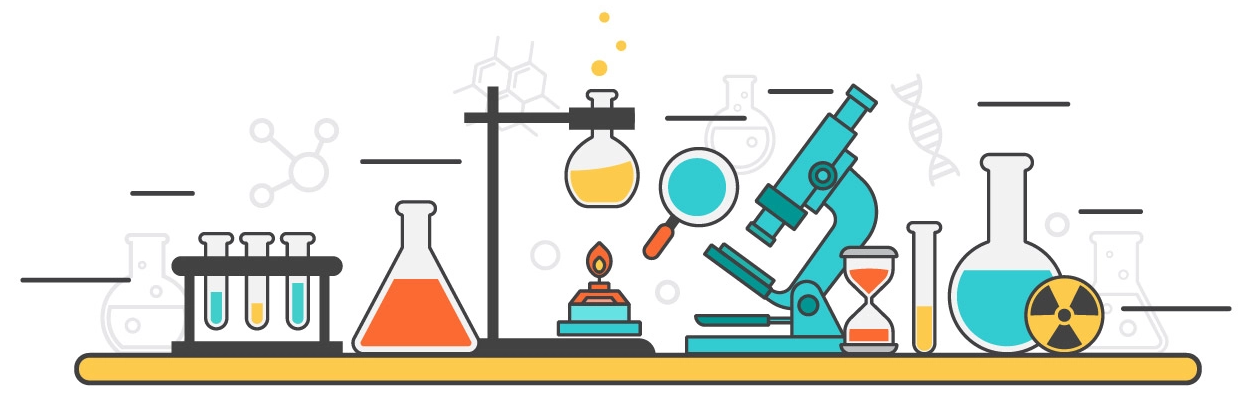
\includegraphics[width=\paperwidth]{../Unidad 2/Images/cover_bg}
\end{document}

\restoregeometry
\addtocontents{toc}{\setcounter{tocdepth}{3}}
\tableofcontents
\chapter{}
%\pagestyle{fancy}
\newpage
\section{Nuestro mundo químico}
\subsection{La química en tu vida y el medio ambiente }

\newpage
\section{Los materiales, las sustancias y sus propiedades}
This is a sample of a section
\subsection{¿Cómo sabemos que un material es distinto de otro?}
\subsection{¿Cómo podemos medir las propiedades de los materiales?}
\newpage
\section{Relación entre propiedades de las sustancias e intercambios de energía}
\subsection{¿Cómo utilizamos energía para analizar sustancias?}

\newpage
\section{Mezclas: propiedades y métodos de separación}

\subsection{Propiedades y clasificación de las mezclas}

\newpage
\section{Mezclas y sustancias contaminantes}
\subsection{¿Cómo detectamos y prevenimos la presencia de sustancias nocivas en el medio ambiente?}

\subsection{Métodos de separación de mezclas}

\newpage
\section{Sustancias elementales y sus propiedades}
\subsection{¿Hay sustancias más simples que otras?}
\subsection{Regularidades en las propiedades de las sustancias elementales}

\chapter{}

\newpage
\section{La estructura de la materia y sus modelos}
\subsection{¿Cómo los átomos y las moléculas hacen distintas a las sustancias?}
\subsection{¿Qué hace a un átomo diferente de otro?}
\subsection{¿Cómo estudiamos a los átomos de manera experimental?}

\newpage
\section{Composición y estructura de distintos tipos de sustancias}
\subsection{¿Qué tipos de partículas se forman al combinar los átomos?}

\newpage
\section{Moléculas de importancia para la vida}
\subsection{¿Qué moléculas nos constituyen?}

\newpage
\section{Relaciones entre la estructura y las propiedades de las sustancias}
\subsection{¿Cómo interaccionan las moléculas?}
\subsection{¿Cómo se explican y predicen las propiedades de las sustancias?}

\newpage
\section{Reacciones químicas en nuestro mundo}
\subsection{¿Cuál es la evidencia de que las sustancias reaccionan unas con otras?}

\newpage
\section{Recombinaciones atómicas}
\subsection{¿Cómo representamos las reacciones químicas?}
\subsection{¿Qué cambia y qué se conserva durante las reacciones químicas?}

\newpage
\section{Cantidad de las sustancias}
\subsection{¿Cómo determinamos la cantidad de las sustancias?}
\subsection{Cantidad de las sustancias en reacciones químicas}


\chapter{}

\newpage
\section{Un mundo de reacciones químicas}
\subsection{¿Cómo nos afectan las reacciones químicas?}
\subsection{¿Cómo aprovechamos las reacciones químicas?}

\newpage
\section{Energía y reacción química}
\subsection{¿Cómo se transfiere energía durante las reacciones químicas?}
\subsection{¿Por qué se transfiere energía durante las reacciones químicas?}

\newpage
\section{La energía química en nuestras vidas}
\subsection{¿Cuáles son los beneficios, costos y riesgos de usar energía química?}

\newpage
\section{Aporte calórico de los alimentos}
\subsection{¿De dónde proviene la energía que necesitamos para vivir?}

\newpage
\section{Rapidez de reacción}
\subsection{¿Qué factores afectan la rapidez de las reacciones químicas?}

\newpage
\section{La rapidez de reacción y el modelo cinético de partículas}
\subsection{¿Cómo explicamos diferencias en la velocidad de reacción?}

\newpage
\section{Utilidad de controlar la rapidez de las reacciones}
\subsection{¿Cómo controlamos y aprovechamos la velocidad de reacción?}

\end{document}